% ---------------------------------------------------------------------
% Jev page triage: paste into the System Design section (after Parsing).
% Needs: \usepackage{booktabs} (acmart loads it), jev-sorter.png uploaded,
% No bibliography entries needed in this version.
% ---------------------------------------------------------------------
\subsection{Page triage with Jev}
\label{sec:jev-triage}
A production of several thousand pages is padded with fax covers, records
certifications, release forms and bills. Triage decides how much work each
page gets before the page agent, the most expensive stage, runs
(Figure~\ref{fig:jev-sorter}). It never removes a page: every page stays
indexed and searchable. Its rule is asymmetric on purpose. Reading an
administrative page in full wastes a few cents; holding back a clinical
page can lose the entry that decides a case, such as a fax cover on which
a nurse wrote ``patient called reporting new numbness.''

\paragraph{Jev.} Triage questions go to Jev (TypeSafe, jev-1.13.0,
pinned)\footnote{\url{https://docs.typesafe.ai/models}}, a hosted decision model that answers a
typed choice question with one of the allowed options and a probability
for every option. The answer is always a valid label, the probability is a
routing signal, and several questions fit in one request at
USD~0.042 per million input tokens. Jev only ever selects a label; it never
supplies text that enters the chronology.

\paragraph{How a page is sorted.}
\begin{enumerate}
\item \emph{Duplicates, in code.} Stamps (Bates numbers, ``page 3 of 12'',
  fax lines) are removed, and a page whose five-word shingles are at least
  90\% contained in an earlier page (Broder's containment measure) is linked
  to it. A copy that adds more than three words, or any clinical word, is
  treated as an amended note and read.
\item \emph{Reuse, in code.} A known form, a run of bills, or a page with
  the same header as the previous page of its document reuses the earlier
  answer, with a Jev spot check on every fourth page.
\item \emph{A glance to Jev.} Jev sees the top quarter of the cleaned page
  and its position (``page 2 of 3 in its document'') and answers three
  questions: the page type (20 labels), whether it holds clinical notes, only
  a table of values, or nothing clinical, and whether it starts a document.
\item \emph{Uncertain pages.} A type below its bar (0.9 for types that can
  hold a page back, 0.7 for types always read) borrows a confident
  neighbor's type within the same document or is asked again with more
  context; a page still unsure is read in full.
\item \emph{Two keys and safety nets.} A page is held back only if, on its
  \emph{full} text, Jev is confident both that it is an administrative type
  and that it has no clinical content, no clinical keyword appears, and the
  text is clean enough to trust. Bills, medication lists and lab tables go
  to table readers in code. Every other page, including any page where Jev
  fails, is read in full.
\end{enumerate}
Productions are often merged PDFs, so code also finds where each document
starts inside a file (page counters, new titles, letter openings,
``continued'' markers), at precision 1.00 and recall 0.94 on our test
files; Jev's answer may add a start but never remove one.

\begin{figure*}[t]
  \centering
  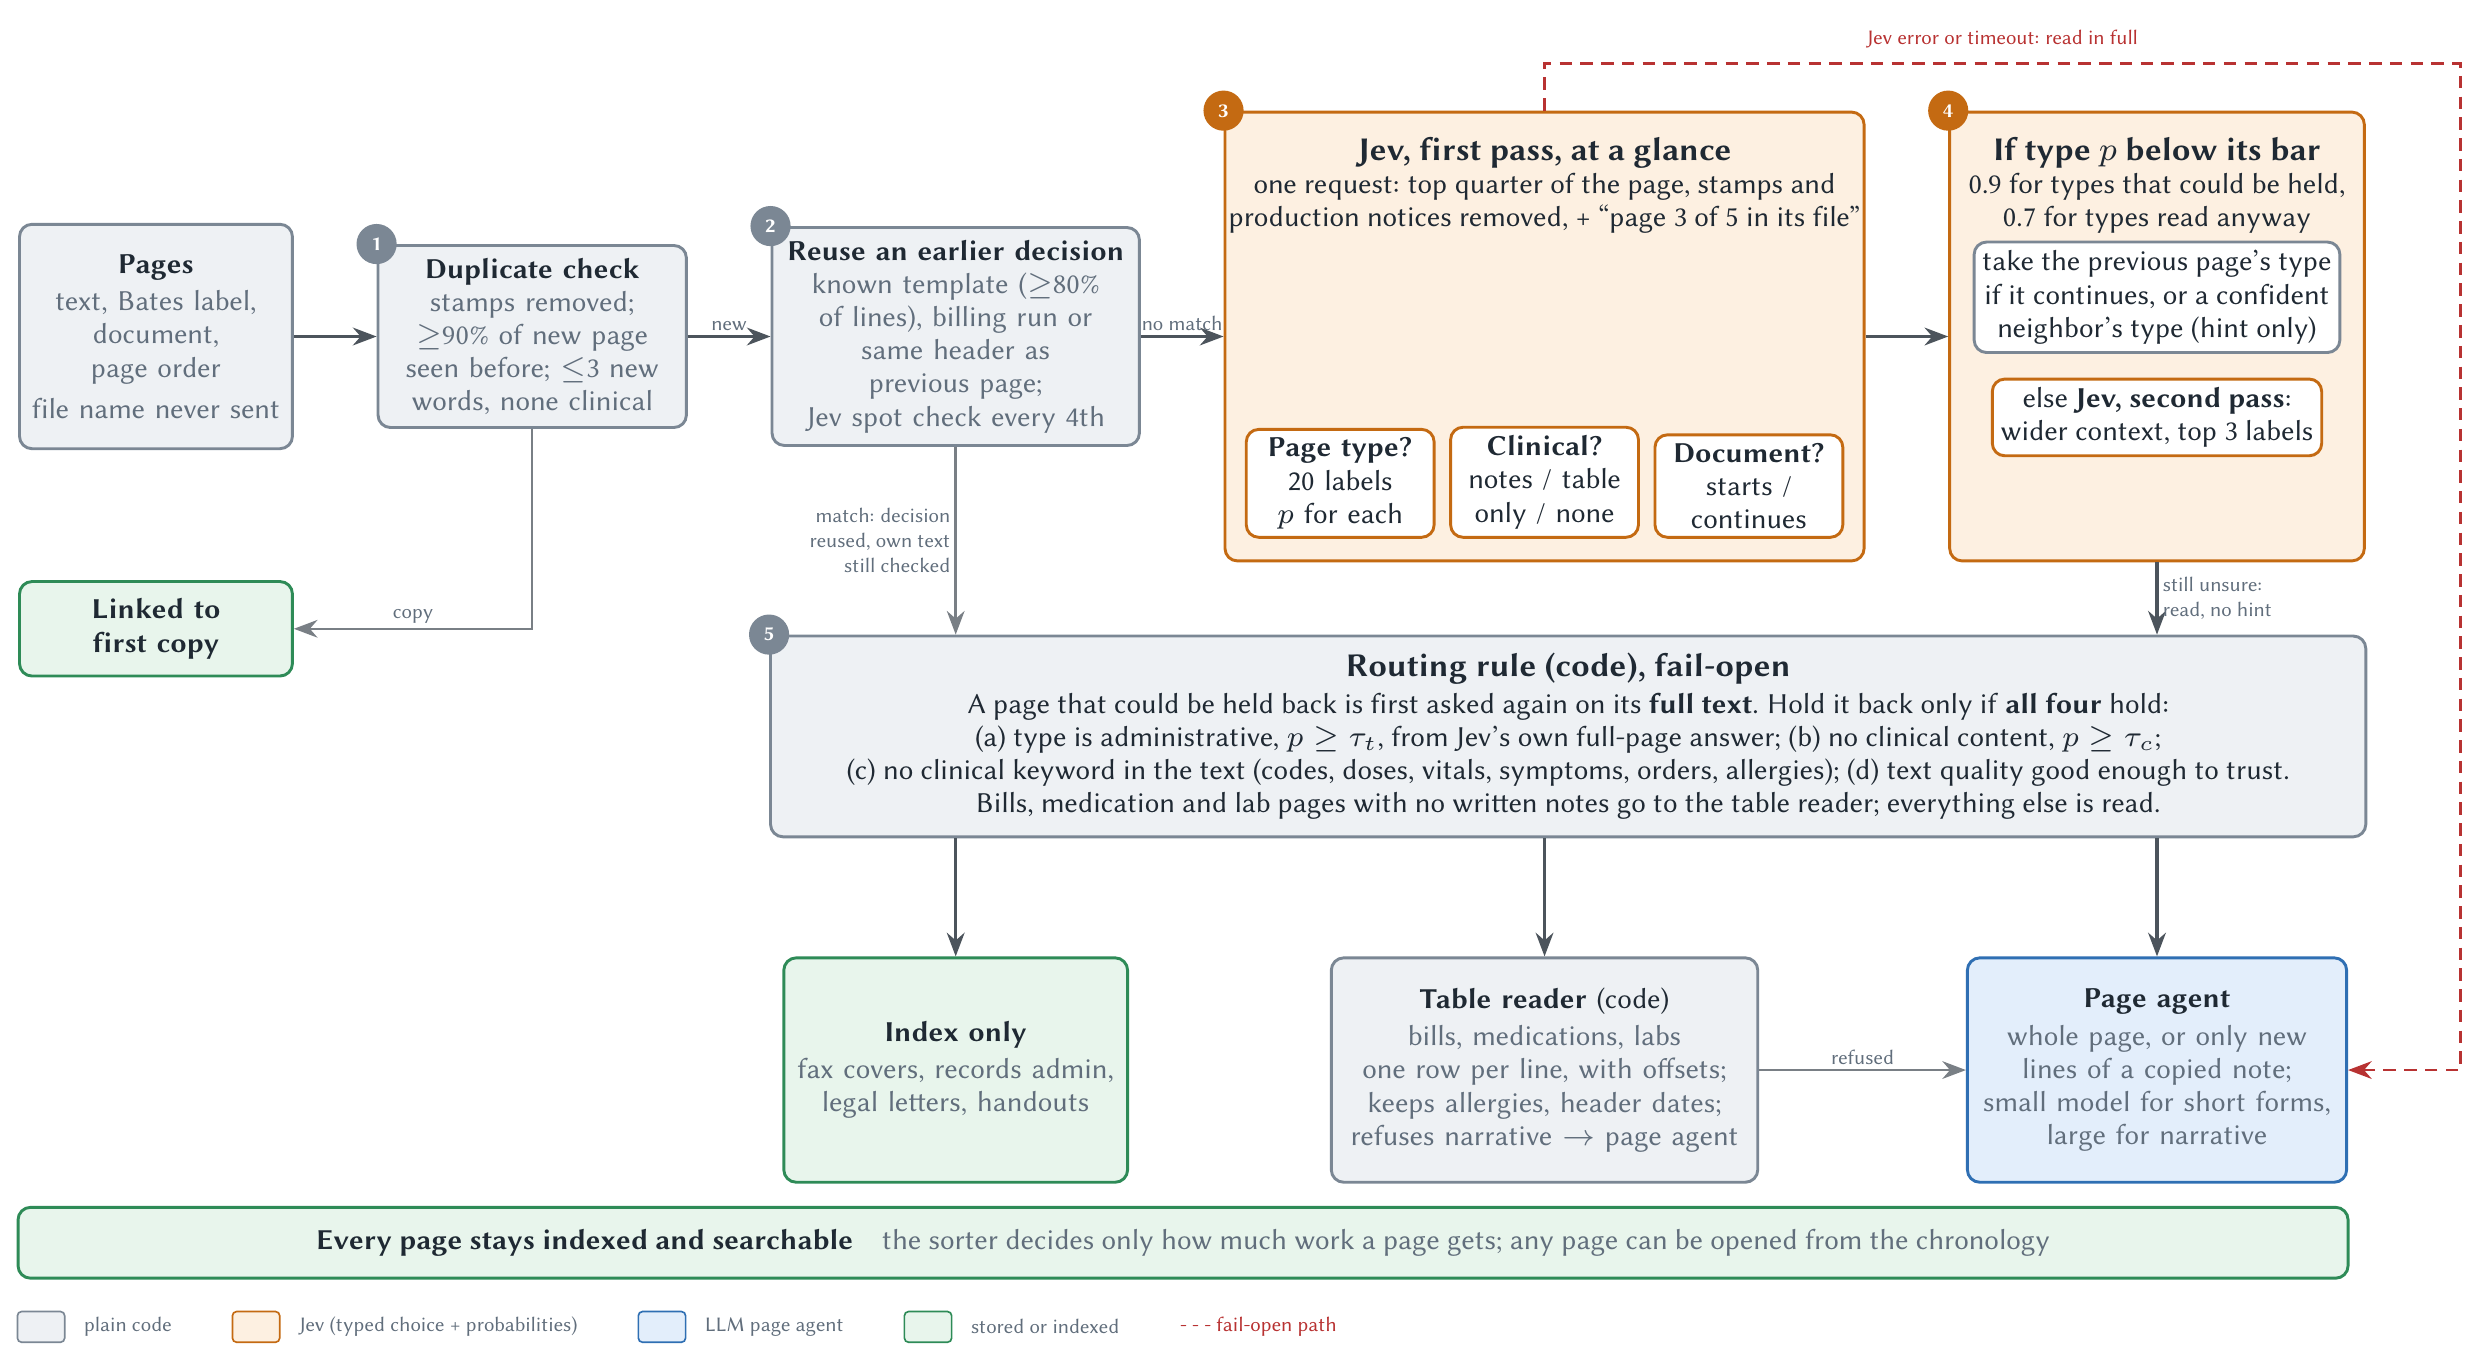
\includegraphics[width=\textwidth]{jev-sorter.png}
  \Description{Schematic of the Jev page sorter: duplicate and reuse checks in code, a glance to Jev with three typed questions, borrowing or re-asking for uncertain pages, and a two-key routing rule with code safety nets that sends each page to index only, a table reader, or the page agent.}
  \caption{The Jev page sorter. Grey steps are code and orange steps are
    Jev requests. A page is held back from a full read only when Jev's
    answers to both questions are confident on the full page and both code
    checks pass; every other page, including any page Jev fails on, goes to
    the page agent.}
  \label{fig:jev-sorter}
\end{figure*}

\subsection{Testing Jev triage}
\label{sec:jev-testing}
All tests use synthetic pages with invented patients; no real record has
been sent to Jev, and none will be until TypeSafe enables zero data
retention. We built five sets: 77 pages used for design, two held-out sets
(32 pages, and 28 pages in multi-page files), 278 pages in 113 files that
were never used for tuning, and 347 generated pages split by file into
tuning and test halves. Each page carries its type, whether it holds
clinical content and whether it starts a document. We also re-ran sets
with injected instructions, OCR noise and production notices added.

\begin{table}[t]
  \caption{Jev triage on synthetic pages (jev-1.13.0). Each cell: pages
    left uncertain / confident types correct / clinical pages held back.
    v5 is the earlier design; v7, the default, adds five labels, a per-type
    confidence bar and the page-position clue.}
  \label{tab:jev-results}
  \small
  \begin{tabular}{@{}lrr@{}}
    \toprule
    Set (pages) & v5 & v7 \\
    \midrule
    Design (77) & 1 / 76 of 76 / 0 & 0 / 77 of 77 / 0 \\
    Held-out 1 (32) & 10 / 21 of 22 / 0 & 3 / 29 of 29 / 0 \\
    Held-out 2 (28) & 6 / 21 of 22 / 0 & 0 / 27 of 28 / 0 \\
    Written, never tuned (278) & 34 / 219 of 244 / 0 & 17 / 251 of 261 / 0 \\
    Generated, test half (174) & 15 / 153 of 159 / 0 & 1 / 170 of 173 / 0 \\
    \bottomrule
  \end{tabular}
\end{table}

\paragraph{Results.} Table~\ref{tab:jev-results} gives the main results.
No run held back a clinical page, including runs with injected
instructions and OCR noise. The changes that mattered most were measured
one at a time. Reading only the top quarter of each page cut the text Jev
reads to about a quarter while keeping 69 of 70 confident answers correct;
adding the last line made results worse. Removing stamps and repeated
production notices before Jev reads a page cut uncertain pages from 21\%
to 4\%. Five extra labels were the largest single gain on the held-out
pages, and the position clue fixed an ED continuation page that every
other version called an office visit with $p=1.00$. Asking each question
twice with the options reversed doubled the cost and caught nothing.
End to end on 75 synthetic PDFs (182 pages), the pipeline held back no
clinical page, typed 170 of 174 pages correctly or as uncertain, and sent
the page agent 48\% of the characters at 0.92 Jev calls per page, about
USD~0.01 in all.

\paragraph{Limits.} Across every set, v7 held back 63 pages and none
were clinical, but zero misses in 63 still allows a true miss rate of
about 5\% at 95\% confidence. The one failure we can produce is
truncation: when OCR drops the only clinical line on an administrative
page, no step can see it. Our pages are also cleaner than real ones. The
first real case (about 60 pages) will therefore be run with a person
checking every page the page agent does not read in full against the PDF.
